\documentclass[aspectratio=169,usenames,dvipsnames]{beamer}
\usepackage{preamble}
\title{Coding for Humanities, week 2}
\begin{document}

\begin{frame}
    \titlepage
\end{frame}

\begin{frame}{Plan for today}
    \tableofcontents
\end{frame}

\begin{frame}{Motivation}
    Until now:
    \begin{itemize}
        \item Work with simple values (numbers, text)
        \item Formulas, arithmetic
        \item Store results in memory (variables)
    \end{itemize}

    \pause
    Today:
    \begin{itemize}
        \item Indexing and slicing strings/lists
        \item Create complex values (\texttt{list})
        \item Making decisions (\texttt{if})
        \item Repetition (\texttt{for})
    \end{itemize}
\end{frame}

\section{Strings}
\frame{\tableofcontents[currentsection]}

\begin{frame}{Strings}
    \begin{definition}
        A \structure{string}, short for string of characters,
        is a type of value that contains text.
    \end{definition}

\end{frame}

\begin{frame}[fragile]{Operations on strings}
\begin{lstlisting}
In: first = 'John'
In: last = 'Doe'
\end{lstlisting}
\begin{description}
    \item[first + last] \texttt{'JohnDoe'}
    \item[first - last] TypeError
    \item[first * last] TypeError
    \item[first / last] TypeError
\end{description}

\begin{itemize}
\item + can be used to concatenate two strings
\item The other operations require numbers, not text
\end{itemize}
\end{frame}

\begin{frame}[fragile]{Mixing strings and numbers}
\begin{lstlisting}
In: first = 'John'
In: num = 3
\end{lstlisting}
\begin{description}
    \item[first + num] TypeError
    \item[first - num] TypeError
    \item[first * num] 'JohnJohnJohn'
    \item[first / num] TypeError
\end{description}

\begin{itemize}
\item * can be used to repeat a string several times
\item For the other operations, Python refuses to mix up types
\end{itemize}
\end{frame}

\begin{frame}[fragile]{Special characters in strings: `escape sequences'}
\begin{lstlisting}
In: print("John's bike")
John's bike
In: print('John\'s bike')  # single quote
John's bike
In: print('John\tMary')  # tab
John    Mary
In: print('John\nMary')  # new line
John
Mary
In: print('Backslash: \\')
Backslash: \
In: print('up\down') # \d is not defined, so backslash is kept
up\down
In: print("\U0001F923", "\N{grinning face}") 
[rolling on the floor laughing and grinning emojis ...]
\end{lstlisting}
\end{frame}

\begin{frame}[fragile]{Indexing: extracting one element}
\begin{lstlisting}
In: name = 'John'
In: name[0]
Out: 'J'
In: name[-1]
Out: 'n'
\end{lstlisting}
    \begin{itemize}
        \item \texttt{a[n]} gets the n'th character of a
        \item Counting starts at 0
        \item negative indices start from the end:\\
			-1 for last character, \\
            -2 second to last, etc.
    \end{itemize}
\end{frame}

\begin{frame}[fragile]{Slicing: extracting a range of elements}
\begin{lstlisting}
In: name = 'John'
In: name[1:3]
Out: 'oh'
In: name[:2]
Out: 'Jo'
In: name[1:]
Out: 'ohn'
\end{lstlisting}
    \begin{itemize}
        \item \texttt{a[n:m]} extracts characters n to m
        \item Counting starts at 0
        \item Result is up to but not including character m \\
                (half-open interval)
        \item if n or m is left out, beginning or end is used
    \end{itemize}
\end{frame}


\begin{frame}
    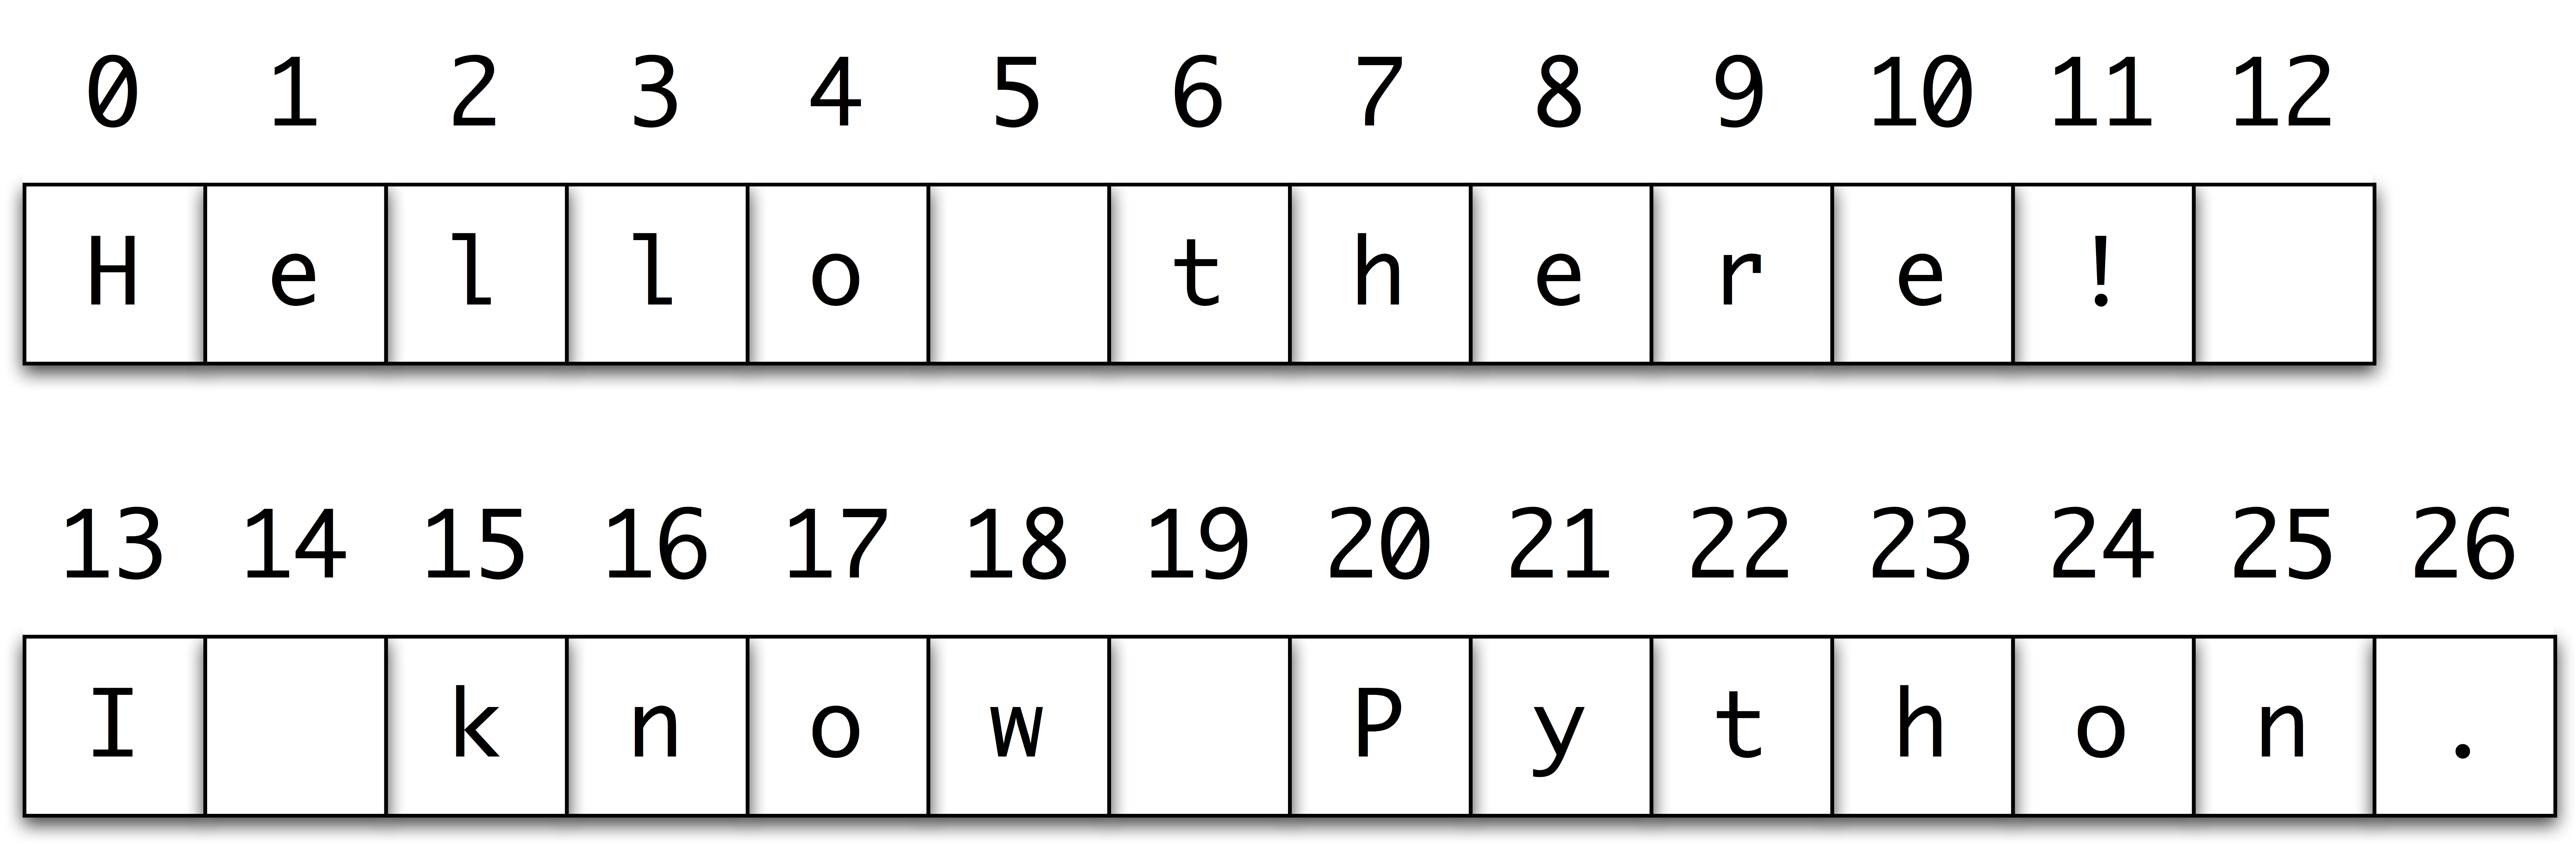
\includegraphics[width=0.8\textwidth]{fig/indexing}
\end{frame}

\begin{frame}[fragile]{Length}
Get the number of characters in a string:
\begin{lstlisting}
In: name = 'John'
In: len(name)
Out: 4
\end{lstlisting}
\end{frame}

\begin{frame}[fragile]{Format strings}
How to combine text and variables in a message?
\begin{lstlisting}
In: x = 1
In: y = 2
In: z = x +  y
In: print("The sum of " + str(x) + " and " + str(y) + " is " + str(z) + ".")
The sum of 1 and 2 is 3.
In: print("The sum of", x, "and", y, "is", z, ".")
The sum of 1 and 2 is 3 .
\end{lstlisting}

\pause
Better:
\begin{lstlisting}
In: print("The sum of {0} and {1} is {2}.".format(x, y, z))
The sum of 1 and 2 is 3.
In: print(f"The sum of {x} and {y} is {z}.")
The sum of 1 and 2 is 3.
\end{lstlisting}

Simple is better, last method is best.
\end{frame}

\begin{frame}{Sequences}
    Strings are a kind of \structure{sequence}
    consisting of characters.

    \vspace{1em}
    A sequence contains elements in a particular order

    \vspace{1em}
    Basic operations on sequences:
    \begin{description}[concatenation:]
        \item[getting length:]     \texttt{len(seq)}
        \item[indexing:]           \texttt{seq[expression]}
        \item[slicing:]            \texttt{seq[start:end]}
        \item[concatenation:]      \texttt{seq1 + seq2}
        \item[repetition:]         \texttt{seq * num}
    \end{description}
\end{frame}


\section{Lists}
\frame{\tableofcontents[currentsection]}

\begin{frame}[fragile]{Lists}
    \begin{definition}
    Lists are sequences that may contain any kind of value as items
    \end{definition}
\begin{lstlisting} 
In: numbers = [0, 1, 2]
In: names = ['John', 'Mary']
\end{lstlisting} 
\end{frame}

\begin{frame}[fragile]{Changing items}
\begin{lstlisting} 
In: names = ['John', 'Mary']
In: names[1] = 'Alice'
In: names
Out: ['John', 'Alice']
\end{lstlisting} 

\pause
NB: cannot change characters in a string (must make new string)
\begin{lstlisting} 
In: name = 'Maria'
In: name[0] = 'D'
TypeError: 'str' object does not support item assignment
\end{lstlisting}

Lists are mutable, strings are immutable:
\begin{definition}
An \structure{immutable} object cannot be changed after it is created.
\end{definition}
\end{frame}

\begin{frame}{Why immutable vs mutable?}
    \begin{description}
        \item[Immutable]
            \begin{itemize}
                \item Easier to reason about:\\
                    created once, never modified
                \item Constant values sometimes required\\
                    (dictionaries, next lecture)
            \end{itemize}

        \item[Mutable]
            \begin{itemize}
                \item More efficient with many changes
                \item More 'natural'
            \end{itemize}
    \end{description}
\end{frame}

\begin{frame}{Objects, methods}
    In Python, every value is an object:

    \begin{definition}
        An \structure{object} encapsulates
        data and code for dealing with that data.

        A function that belongs to and operates on an object
        is called a \structure{method}.
    \end{definition}
   
    \begin{description}
        \item[Regular function:] \texttt{func(a, ...)}
        \item[Method:] \texttt{obj.func(a, ...)}
    \end{description}
\end{frame}

\begin{frame}[fragile]{Adding items}
We can add an item to the end of an existing list:
\begin{lstlisting} 
In: names = ['John', 'Mary']
In: names.append('Alice')
Out: ['John', 'Mary', 'Alice']
\end{lstlisting}

\pause
We can combine two lists into a new list:
\begin{lstlisting} 
In: friends = ['John', 'Mary']
In: enemies = ['Alice', 'Bob']
In: friends + enemies
Out: ['John', 'Mary', 'Alice', 'Bob']
\end{lstlisting}
\end{frame}


\begin{frame}[fragile]{Removing items}
We can remove an item anywhere in a list:
\begin{lstlisting} 
In: names = ['John', 'Mary']
In: names.remove('John')
Out: ['Mary']
\end{lstlisting}

\texttt{remove(elem)} \structure{searches} for the first occurrence of
\texttt{elem} and removes it.

\pause
\vspace{1em}
Can also remove items at particular positions:
\begin{lstlisting} 
In: acquaintances = ['John', 'Mary', 'Alice', 'Bob', 'Max']
In: acquaintances.pop(3)  # removes 4th item
In: acquaintances.pop()   # removes last item
In: friends = acquaintances[:2]  # new list from slice
In: friends
Out: ['John', 'Mary']
\end{lstlisting}

% We can also use slicing to keep a part of a list
% \begin{lstlisting} 
% In: acquaintances = ['John', 'Mary', 'Alice', 'Bob']
% In: friends = acquaintances[:2]
% In: friends
% Out: ['John', 'Mary']
% \end{lstlisting}
%This is faster if you know where the items are that you want to keep.
\end{frame}


\begin{frame}[fragile]{The split method}
We can turn a string into a list of strings
by splitting on a character:
\begin{lstlisting} 
In: quote = "Frankly, my dear, I don't give a damn."
In: quote.split(",")
Out: ['Frankly', ' my dear', " I don't give a damn."]
\end{lstlisting}

\pause
If we don't give a character, splits on whitespace:
\begin{lstlisting} 
In: quote.split()
Out: ['Frankly,', 'my', 'dear,', 'I', "don't", 'give', 'a', 'damn.']
\end{lstlisting}
\end{frame}


\begin{frame}[fragile]{Sorting}
\begin{lstlisting} 
In: letters = list('ocd')
In: letters
Out: ['o', 'c', 'd']
In: sorted(letters)
Out: ['c', 'd', 'o']
\end{lstlisting}

NB: sorted leaves the original list unchanged,
assign it to keep the result.
\end{frame}

\begin{frame}[fragile]{Putting a list of strings back together as one string}
\begin{lstlisting}
In: ''.join(sorted(letters))
'cdo'
\end{lstlisting}
Equivalent of:
\begin{lstlisting}
In: 'c' + '' + 'd' + '' + 'o'
\end{lstlisting}

\texttt{sep.join(seq)} is the opposite of \texttt{str.split(sep)}
\end{frame}


\begin{frame}[fragile]{Nested lists}
    \begin{columns}
        \column{0.3\linewidth}
            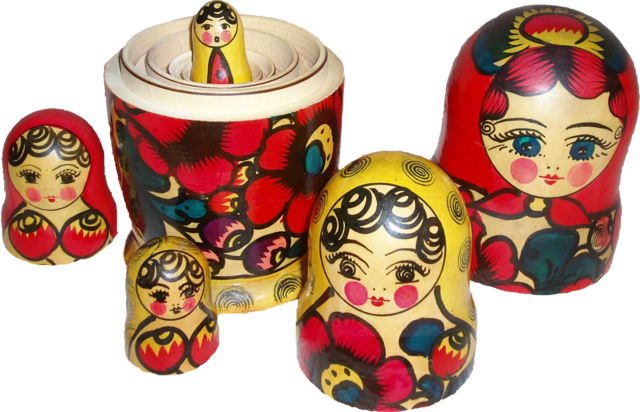
\includegraphics[width=0.95\textwidth]{fig/russiandolls}

            {\scriptsize
            (from \href{https://en.wikipedia.org/wiki/Matryoshka_doll#/media/File:Matryoshka_transparent.png}{Wikipedia})}
        \column{0.7\linewidth}
            Can put lists inside of lists \dots
\begin{lstlisting}
In: ranking = [['John', 1], ['Mary', 3], ['Max', 2]]
\end{lstlisting}

\pause
How to access elements:
\begin{lstlisting}
In: name_and_rank = ranking[0]
Out: ['John', 1]
In: name_and_rank[1]  # extract rank
Out: 1
In: ranking[0][1]  # can also get rank directly
Out: 1
In: name, rank = name_and_rank
\end{lstlisting}
    \end{columns}
\end{frame}

\begin{frame}[fragile]{Summary: strings vs lists}
Both strings and lists are sequences:
    \begin{itemize}
        \item Items in a fixed order
        \item Has a length
        \item Can extract items or slices
    \end{itemize}

Two important differences:
\begin{enumerate}
    \item lists are more general than strings
        \begin{itemize}
            \item Strings always consist of characters
            \item Lists can consist of any data types / objects
        \end{itemize}
    \item Lists are mutable and strings are immutable
\end{enumerate}

    Convert between strings and lists:
        \texttt{list(), .split(), .join()}
\end{frame}







\section{Conditional statements: do you really want to do that?}
\frame{\tableofcontents[currentsection]}

\begin{frame}{Making decisions: flow charts}
    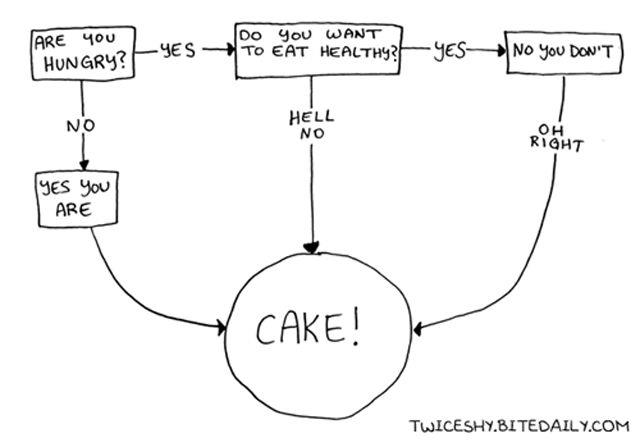
\includegraphics[height=0.8\textheight]{fig/flowchart}
\end{frame}


\begin{frame}{Simple conditions}
    \begin{definition}
        A \structure{conditional expression} is
        an expression that is \texttt{True} or \texttt{False}
    \end{definition}
    Conditional operators:
    \begin{description}
        \item[a == b] are the values equal?
        \item[a != b] inequality
        \item[a $<$ b] test whether a is strictly smaller than b
        \item[a $>$ b]
        \item[a in b] does element a occur in the sequence b?
    \end{description}

\end{frame}

\begin{frame}{Statements vs expressions}
    NB: == tests equality, \\
           = is an assignment statement!

    \begin{description}
        \item[Statement:] must occur on a new line. \structure{does} something.
        \item[Expression:] may occur in many places, e.g., inside another expression.
            Evaluates to a \structure{value}, usually without changing anything.
    \end{description}
\end{frame}

\begin{frame}[fragile]{The if-statement}
\begin{lstlisting}
if books > 5:
    print('you are an avid reader')
\end{lstlisting}

    \begin{itemize}
        \item The code under an if-statement is only executed
            if the condition is True.
        \item The indentation determines which code is covered
            by the condition
    \end{itemize}

    \pause
    \begin{definition}
        A \structure{code block} is a sequence of indented lines after
        a statement ending in `:'.
        The start and end of the block are defined by the indentation of the
        lines.
    \end{definition}
\end{frame}


\begin{frame}[fragile]{Optional extensions of the if-statement}
\begin{lstlisting}
if books > 5:
    print('you are an avid reader')
else:
    print('you should read more')
\end{lstlisting}

\begin{itemize}
    \item The code under 'else' is executed if the condition does NOT match.
\end{itemize}
\end{frame}


\begin{frame}[fragile]{Optional extensions of the if-statement}
\begin{lstlisting}
if books > 15:
    print('you should get out more')
elif books > 5:
    print('you are an avid reader')
else:
    print('you should read more')
\end{lstlisting}

\begin{itemize}
    \item Can add multiple extra conditions with 'elif' (else if)
    \item The conditions are tested from top to bottom;
            when one of them matches, the rest are ignored.
\end{itemize}
\end{frame}


\begin{frame}[fragile]{Complex conditions}
    Can create complex conditions from other conditions:
    
    \begin{description}
        \item[cond1 and cond2]
        \item[cond1 or cond2]
        \item[not cond]
    \end{description}

    \pause
    For example:
\begin{lstlisting}
if books > 5 and books < 15:
    ...
\end{lstlisting}

\end{frame}

\begin{frame}[fragile]{Truthy and Falsy things}
\begin{itemize}
    \item The number zero and empty sequences are treated as \texttt{False}.
    \item Nonzero numbers and nonempty sequences are treated as \texttt{True}.
\end{itemize}

These are equivalent:
\begin{lstlisting}
if len(booklist) != 0:
    print('yes')    
if len(booklist):
    print('yes')    
if booklist:
    print('yes')    
\end{lstlisting}

    Simple is better, so last one is preferred
\end{frame}

\begin{frame}[fragile]{Converting a decision tree into if-statements}
    \begin{columns}
        \column{0.5\linewidth}
            ``Should you stay at a social gathering?''

            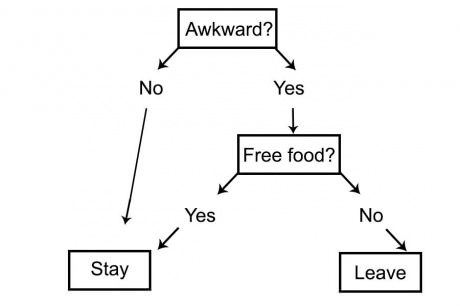
\includegraphics[width=0.8\textwidth]{fig/flowchart2}

        \pause
        \column{0.5\linewidth}
\begin{lstlisting}
awkward = False
free_food = True
if awkward:
    if free_food:
        print('Stay')
    else:
        print('Leave')
else:
    print('Stay')
\end{lstlisting}
\end{columns}
\end{frame}


\begin{frame}{Summary}
    \begin{description}
        \item[Conditions] An expression that is \texttt{True} or \texttt{False}.

                Comparisons, equality tests: <, >, ==, !=

                Complex conditions: \texttt{and, or, not}

        \item[if-statements] Execute statements only if condition is True
    \end{description}
\end{frame}


\section{Loops: play it again, Sam!}
\frame{\tableofcontents[currentsection]}

\begin{frame}[fragile]{Repeating statements: loops}
\begin{lstlisting}
booklist = ['a', 'b', 'c']
for book in booklist:
    print(book)
\end{lstlisting}
Result:
\begin{lstlisting}
a
b
c
\end{lstlisting}

\begin{itemize}
\item The statements under the for-loop are repeated \\
    for every element in the sequence.
\item At every iteration, 'book' is assigned an element of 'booklist'
\end{itemize}
\end{frame}

\begin{frame}[fragile]{Looping over sequences}
For loops can be used for anything with multiple items (\structure{iterable}):
\begin{lstlisting}
for letter in 'word':
    print(letter)
for number in [0, 1, 2]:
    print(number)
\end{lstlisting}
\end{frame}



\begin{frame}[fragile]{Looping without a list}
Can use the \texttt{range} function if we don't have a list:
\begin{lstlisting}
for number in range(4):
    print(number)
\end{lstlisting}

Result:
\begin{lstlisting}
0
1
2
3
\end{lstlisting}

Repeats 4 times. Last item is 3 because counting starts at 0.
\end{frame}

\begin{frame}{Summary}
    \begin{description}
        \item[for-loop] repeat code for each element
        \item[iterables] strings, lists, range
        %\item[]
    \end{description}
\end{frame}

\begin{frame}{Summary of today}
    \begin{description}
        \item[Strings] text
        \item[Lists] 
        \item[Conditions] if-statement
        \item[Repetition] for-loop
    \end{description}
\end{frame}


\begin{frame}{Background reading}
    \begin{itemize}
        \item Downey ch.\ 5, 8, 10
        \item and/or Zelle sec.\ 5.1-5.8
        \item Watch youtube tutorials of "Hacking the Humanities" episode 6--9:
            \url{https://www.youtube.com/playlist?list=PL6kqrM2i6BPIpEF5yHPNkYhjHm-FYWh17}
    \end{itemize}
\end{frame}
\end{document}
